
%(BEGIN_QUESTION)
% Copyright 2010, Tony R. Kuphaldt, released under the Creative Commons Attribution License (v 1.0)
% This means you may do almost anything with this work of mine, so long as you give me proper credit

Determine what pressure conditions must be met at each of the four pressure switches in order for the lamp to energize:

$$\includegraphics[width=15.5cm]{i00019x01.eps}$$

\noindent
Trip settings for each pressure switch:

\begin{itemize}
\item{} PS1 = 50 PSI
\item{} PS2 = 31 PSI
\item{} PS3 = 77 PSI
\item{} PS4 = 8 PSI
\end{itemize}

\vfil

\underbar{file i00019}
\eject
%(END_QUESTION)





%(BEGIN_ANSWER)

This is a graded question -- no answers or hints given!

%(END_ANSWER)





%(BEGIN_NOTES)

The major principle to keep in mind here is that the lamp can only receive power through {\it closed} switch contacts.  Therefore, we must look for conditions necessary to make each switch contact close.  If the switch in question is NO, pressure above the trip value must be applied to close it.  If the switch in question is NC, it will already be closed if pressure is less than the trip value.

\vskip 10pt

(PS1 less than 50 PSI {\it or} PS4 greater than 8 PSI) {\it and} PS2 less than 31 PSI {\it and} PS3 greater than 77 PSI.

%INDEX% Switch, pressure: ladder logic circuit

%(END_NOTES)


